\subsection{Analisi}
Questa fase comincia con la presentazione dei capitolati d'appalto e termina con la data di consegna per la \textit{Revisione dei Requisiti}, ovvero dal 05/11/2020 al 11/01/2021.
In questo periodo verranno redatti tutti i documenti necessari e verrà fatta un'analisi approfondita del capitolato scelto dal gruppo \Gruppo{}.
\subsubsection{Attività}
\begin{itemize}
\item \textbf{\SdF}: viene effettuato uno studio dei capitolati proposti, analizzandone aspetti positivi e negativi al fine d'identificare il capitolato per cui concorrere. Questa attività è bloccante per l'\textit{\AdR} ;
\item \textbf{\NdP}: vengono definite tutte le norme che il gruppo \Gruppo{} seguirà durante lo sviluppo dell'intero progetto;
\item \textbf{\PdP}: il presente documento, in cui le attività, i compiti\glo{} e le risorse precedentemente analizzate vengono distribuite tra i membri del team \Gruppo{}; presenta il calcolo del preventivo per la realizzazione del progetto;
\item \textbf{\AdR}: vengono studiati ed analizzati i requisiti del capitolato\glo{} scelto nello \textit{\SdF};
\item \textbf{\PdQ}: si espongono i metodi necessari e scelti a garantire la qualità del prodotto;
\item \textbf{\Glossario}: vengono definiti in modo conciso i termini che possono risultare ambigui durante lo svolgimento del progetto;
\item \textbf{Lettera di Presentazione}: breve documento in cui il gruppo \Gruppo{} si candida come fornitore del prodotto software richiesto.
\end{itemize}
\subsubsection{Periodi}
La pianificazione di questa fase è stata organizzata nei seguenti periodi:
\begin{itemize}
\item \textbf{Periodo 1}: \textit{(dal 05/11-2020 al 04/12/2020)} scelta del nome e del logo del gruppo, creazione della mail di riferimento e individuazione degli strumenti per la comunicazione interna. Discussione dei capitolati proposti per individuare quello preferito dal gruppo e inizio della stesura dello \textit{\SdF{}} ; iniziato anche il \Glossario. \\Il 10-12-2020 il gruppo ha fissato una milestone\glo{} per la conclusione dello \textit{\SdF{}} e la scelta del capitolato.\\Stesi i verbali interni relativi alle riunioni in questa fase.
\item \textbf{Periodo 2 }: \textit{(dal 05/12/2020 al 22/12/2020)} stesura delle \textit{\NdP{}} e del \textit{\PdP{}} con l'esposizione della pianificazione del lavoro da svolgere nel corso del progetto e la suddivisione dei ruoli tra i membri del gruppo. Iniziata inoltre la stesura dell'\textit{\AdR{}}.\\Il 22/12/2020 il gruppo ha fissato una milestone per verificare che il documento \textit{\NdP{}} sia completato correttamente e valutare come distribuire eventuali ritardi.\\Stesi i verbali interni relativi alle riunioni in questa fase.
\item \textbf{Periodo 3}: \textit{(dal 23/12/2020 al 05/01/2020)} il gruppo si dedica all'\textit{\AdR{}} e al contempo inizia la stesura del \textit{\PdQ{}}, con la seguente esposizione dei criteri di valutazione della qualità scelti dal gruppo e le rispettive metriche\glo{} di calcolo.\\Il 05/01/2020 il gruppo fissa un'ulteriore milestone per verificare che tutti i documenti siano stati completati correttamente e valutare come distribuire eventuali ritardi.\\Continuano le attività di verifica incrementale per i documenti in corso di stesura.\\Stesi i verbali interni relativi alle riunioni in questa fase.
\item \textbf{Periodo 4}: \textit{(dal 06/01/2020 al 11/01/2020)} si svolge attività di verifica su tutti i documenti, si completano eventualmente documenti in ritardo. Si uniformano tutti i documenti stando alle regole stabilite nelle \textit{\NdP{}}. Si scrive inoltre la lettera di presentazione.\\Stesi i verbali interni relativi alle riunioni in questa fase.
\end{itemize}

\newpage
\subsubsection{Diagramma di Gantt: Analisi}
\begin{figure}[h]
	\centering
	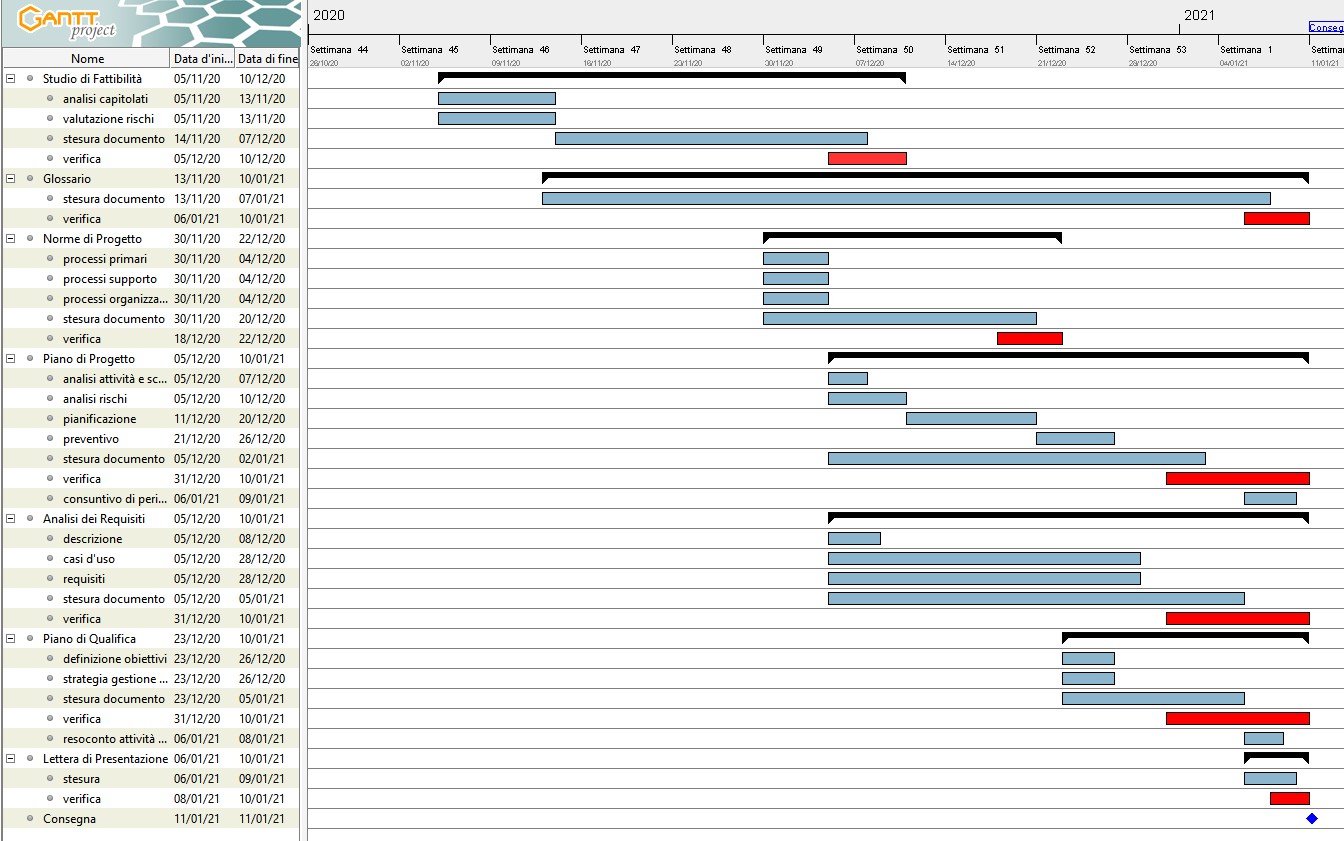
\includegraphics[scale=0.45]{Images/GanttPianificazioneAnalisi.PNG}
	\caption{Diagramma di Gantt dell'attività di Analisi}
\end{figure}